\section{Results}\label{sec:results}

\subsection{Honest operation and the bound check}
The simulator reproduces the expected finite-key behaviour. At the calibration point the honest link yields $\keyrateDZero\times10^{-3}$ secret bits per pulse; nominal drift lowers this to $\keyrateDOne\times10^{-3}$ and fourfold drift to $\keyrateDFour\times10^{-3}$, where \keyposDFour\% of the blocks still produce a key. Over the \nBlocksHonest{} honest blocks the lower bound $s_{Z,1}$ exceeded the true single-photon count \boundViol{} times, and no honest block met the breach condition (\ref{eq:breach}). At $d=1$ the stream loss spans \lossminDOne--\lossmaxDOne\,dB and the misalignment reaches \edmaxDOne\%; at $d=4$ the ranges are \lossminDFour--\lossmaxDFour\,dB and \edmaxDFour\%.

\subsection{False alarms under drift}
Table~\ref{tab:fpr} and Figure~\ref{fig:fpr} give the per-window false-alarm rate on benign streams. Every calibrated detector meets its $10^{-3}$ target at $d=0$. Drift separates them at once. IF-stat and RF-stat alarm in \fprIFstatDOne\% and \fprRFstatDOne\% of benign windows at $d=1$; their alarms track the hourly misalignment cycle (Figure~\ref{fig:trace}, lower panels), so an operator would see a periodic alarm on a healthy link. Domain randomisation helps but does not hold the target: RF-DR reaches \fprRFDRDOne\% at $d=1$ and \fprRFDRDFour\% at $d=4$, with large seed-to-seed spread. IF-drift, fitted on benign drift up to $d=2$, stays at \fprIFdriftDOne\% at $d=1$ and rises to \fprIFdriftDTwo\% and \fprIFdriftDFour\% at $d=2$ and $d=4$. The DCS stays between \fprDCSDOne\% and \fprDCSDFour\% at every scale. Its paired difference from each learned detector at $d\geq1$ has Holm-adjusted $p\leq\holmFprMax$; against the fixed QBER rule, which raised no alarm at all, the DCS is the worse of the two on this metric. Moving the thresholds to drifted calibration data (Table~\ref{tab:fprdcal} in the appendix) brings RF-DR to \fprdcalRFDRDFour\% and IF-drift to \fprdcalIFdriftDFour\% at $d=4$, at the price of benign drift data recorded on the target link.

\begin{table}[t]
\centering
\caption{Per-window false-alarm rate (\%) on 24-hour benign streams, thresholds calibrated on drift-free data for $\alpha=0.1\%$. Mean $\pm$ 95\% $t$-interval over \nSeeds{} seeds.}\label{tab:fpr}
\small\begin{tabular}{lrrrrr}
\hline
Detector & $d=0$ & $d=0.25$ & $d=1$ & $d=2$ & $d=4$\\
\hline
QBER & 0.00 [0.00, 0.00] & 0.00 [0.00, 0.00] & 0.00 [0.00, 0.00] & 0.00 [0.00, 0.00] & 0.00 [0.00, 0.00]\\
Band & 0.10 [0.09, 0.11] & 89.31 [89.06, 89.54] & 97.27 [97.19, 97.34] & 98.65 [98.61, 98.69] & 99.42 [99.40, 99.44]\\
DCS & 0.11 [0.10, 0.13] & 0.11 [0.09, 0.12] & 0.10 [0.09, 0.11] & 0.10 [0.09, 0.11] & 0.10 [0.08, 0.11]\\
CUSUM & 0.15 [0.11, 0.21] & 0.11 [0.08, 0.16] & 0.11 [0.08, 0.15] & 0.11 [0.08, 0.15] & 0.17 [0.12, 0.22]\\
Block & 0.09 [0.07, 0.13] & 0.12 [0.09, 0.17] & 0.10 [0.07, 0.15] & 0.08 [0.05, 0.13] & 0.12 [0.08, 0.18]\\
IF-stat & 0.10 [0.09, 0.11] & 41.52 [39.39, 44.20] & 95.05 [94.60, 95.46] & 99.13 [99.01, 99.23] & 99.88 [99.86, 99.90]\\
IF-drift$^\dagger$ & 0.00 [0.00, 0.00] & 0.00 [0.00, 0.00] & 0.00 [0.00, 0.00] & 0.55 [0.39, 0.81] & 30.71 [28.42, 33.05]\\
IF-res & 0.11 [0.10, 0.13] & 0.10 [0.09, 0.11] & 0.10 [0.08, 0.11] & 0.09 [0.08, 0.11] & 0.08 [0.07, 0.09]\\
RF-stat & 0.09 [0.08, 0.11] & 6.34 [4.76, 8.60] & 74.57 [72.36, 76.65] & 92.92 [92.16, 93.61] & 98.86 [98.66, 99.03]\\
RF-DR$^\dagger$ & 0.00 [0.00, 0.00] & 0.00 [0.00, 0.00] & 0.01 [0.00, 0.05] & 0.64 [0.46, 0.90] & 8.43 [5.27, 13.28]\\
RF-res$^\dagger$ & 0.11 [0.09, 0.12] & 0.11 [0.10, 0.13] & 0.11 [0.09, 0.12] & 0.09 [0.08, 0.11] & 0.08 [0.07, 0.09]\\
DCS-X & 0.10 [0.09, 0.11] & 0.10 [0.09, 0.12] & 0.11 [0.09, 0.12] & 0.10 [0.09, 0.12] & 0.12 [0.11, 0.13]\\
Band-roll$^\dagger$ & 0.00 [0.00, 0.01] & 0.00 [0.00, 0.01] & 0.00 [0.00, 0.01] & 0.69 [0.43, 1.31] & 30.20 [29.05, 31.55]\\
\hline
\end{tabular}
\end{table}

\begin{figure}[t]
\centering
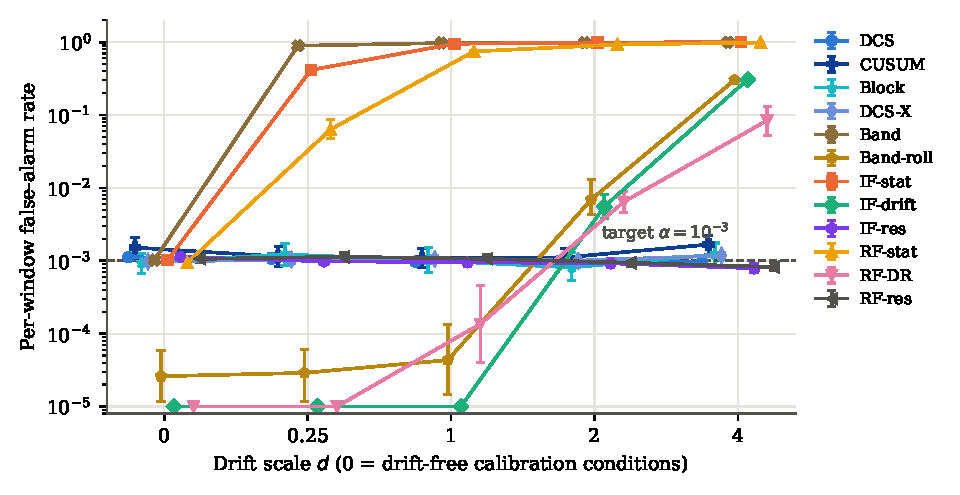
\includegraphics[width=0.62\linewidth]{figures/fpr_vs_drift.pdf}
\caption{Per-window false-alarm rate against drift scale (log axis; error bars are 95\% $t$-intervals over \nSeeds{} seeds). IF-stat (squares) and RF-stat (triangles) overlap near 1 for $d\geq1$. The QBER rule raised no alarms and is not shown on the log axis. The dashed line is the calibration target.}\label{fig:fpr}
\end{figure}

\begin{figure}[t]
\centering
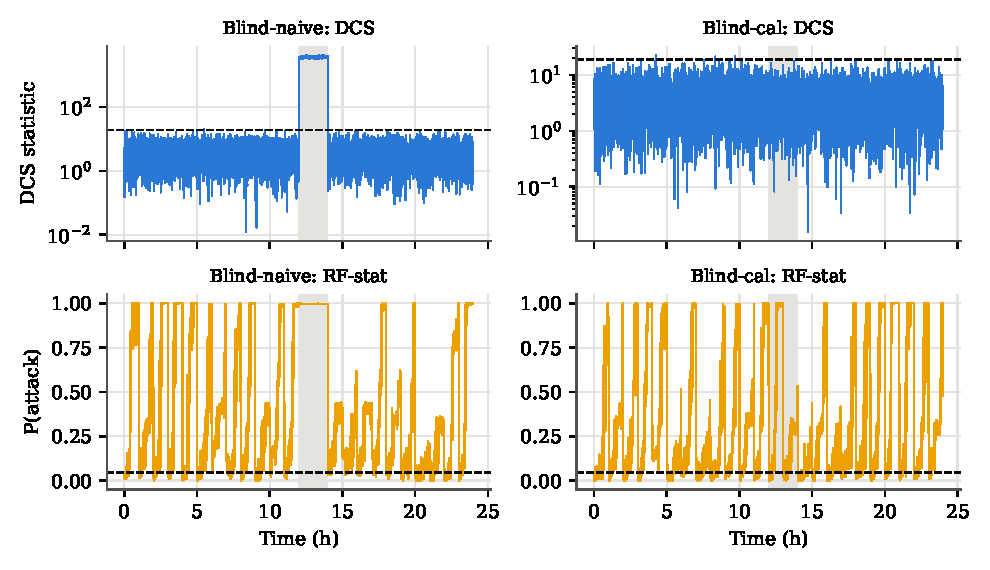
\includegraphics[width=0.92\linewidth]{figures/trace_d1.pdf}
\caption{Window scores over one 24-hour stream at $d=1$ with the attack active in the shaded two hours; dashed lines are the calibrated thresholds. Left: Blind-naive. Right: Blind-cal. Top: DCS (log axis). Bottom: RF-stat, whose score follows the hourly misalignment ramp and crosses its threshold in most benign windows.}\label{fig:trace}
\end{figure}

\subsection{Which attacks are separable}
Figure~\ref{fig:auc} gives the ROC AUC at $d=1$; Table~\ref{tab:aucd0} in the appendix gives $d=0$. Four results stand out.

The calibrated attack is invisible. For Blind-cal the AUC of every detector at every drift scale lies between \aucCalMin{} and \aucCalMax{}, as Proposition~\ref{prop:indist} requires. The high TPR of IF-stat and RF-stat on Blind-cal in Table~\ref{tab:tpr} is their benign false-alarm rate, not detection.

Errors in the attacker's calibration are visible to the DCS when they break a physical relation the refit cannot absorb. Blind-naive (no dark counts, no errors, wrong decoy ratio) and Blind-gain (correct gains, no errors) give AUC 1.00 and an alarm in the first attacked window in every seed and at every drift scale. Blind-nodark is the exception: the refit lowers $\hat Y_0$ to match the missing dark counts and the residuals stay small, so the DCS scores \aucNodarkDCSDOne{} at $d=1$. The learned detectors see this attack (IF-drift \aucNodarkIFdriftDOne{}, RF-DR \aucNodarkRFDRDOne{}) because they compare absolute levels with what they were trained on.

An attacker who ignores drift becomes distinguishable in the opposite direction. Blind-cal-static emits the statistics of the nominal channel while the real channel drifts. The learned detectors score these windows as \emph{more} normal than the benign ones (IF-stat AUC \aucStaticIFstatDOne{}, RF-stat \aucStaticRFstatDOne{} at $d=1$), so the drift itself is the signature, but only a detector that alarms on missing variation would use it. The DCS, which refits every window, scores \aucStaticDCSDOne{}.

In-model attacks are detected but do not need to be. IR and PNS give DCS AUC near 1 at every drift scale; at $d=0$ the learned detectors reach AUC between \aucInModelLearnedMin{} and 1.00 on the same attacks. The DCS cannot see added loss (AUC below 0.5) by construction.

\begin{figure}[t]
\centering
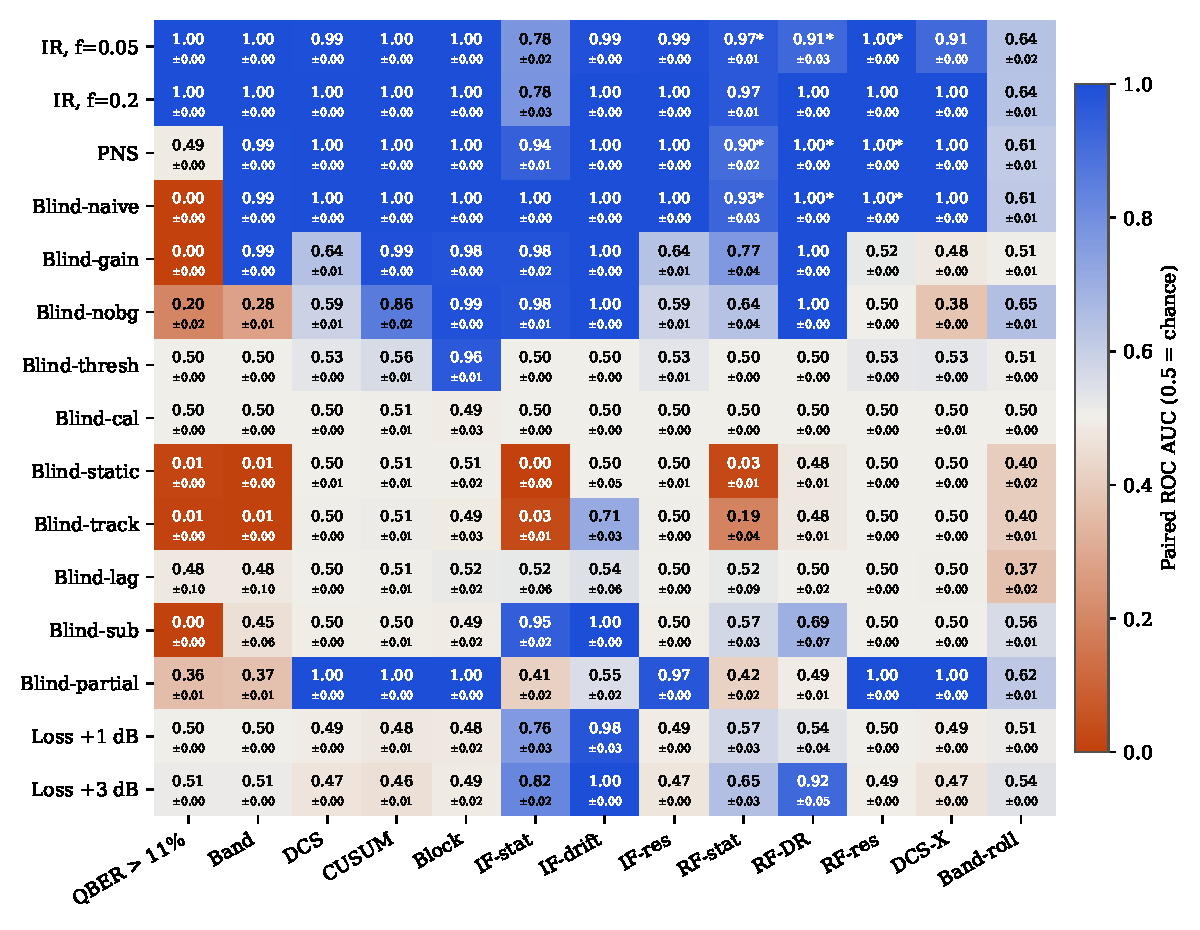
\includegraphics[width=0.72\linewidth]{figures/auc_heatmap_d1.pdf}
\caption{ROC AUC at $d=1$ (mean over \nSeeds{} seeds). Blue: attack windows score higher than benign windows; orange: lower; light grey: chance. Values below 0.5 for the static calibrated attack mean that its windows look more stationary than the drifting benign windows.}\label{fig:auc}
\end{figure}

\begin{table}[t]
\centering
\caption{TPR at the drift-free calibrated threshold, $d=1$ (mean over \nSeeds{} seeds). The first row is the benign FPR of the same detector; a TPR close to it is not detection.}\label{tab:tpr}
\small\begin{tabular}{lcccccc}
\hline
Attack & QBER$>$11\% & DCS (ours) & IF-stat & IF-drift & RF-stat & RF-DR\\
\hline
\emph{benign FPR} & 0.000 & 0.001 & 0.972 & 0.003 & 0.975 & 0.092\\
IR, $f=0.05$ & 0.000 & 0.946 & 1.000 & 0.560 & 1.000 & 0.883\\
IR, $f=0.2$ & 0.000 & 1.000 & 1.000 & 1.000 & 1.000 & 1.000\\
PNS & 0.000 & 1.000 & 1.000 & 1.000 & 1.000 & 1.000\\
Blind-naive & 0.000 & 1.000 & 1.000 & 1.000 & 1.000 & 0.997\\
Blind-gain & 0.000 & 1.000 & 1.000 & 0.997 & 1.000 & 0.969\\
Blind-nodark & 0.000 & 0.002 & 1.000 & 0.940 & 1.000 & 0.846\\
Blind-cal & 0.000 & 0.001 & 0.974 & 0.003 & 0.976 & 0.054\\
Blind-cal-static & 0.000 & 0.001 & 0.001 & 0.001 & 0.000 & 0.001\\
Loss +1 dB & 0.000 & 0.000 & 0.997 & 0.707 & 1.000 & 0.875\\
Loss +3 dB & 0.000 & 0.001 & 1.000 & 1.000 & 1.000 & 1.000\\
\hline
\end{tabular}
\end{table}

\subsection{Finite-key audit}
Table~\ref{tab:key} links detection to secrecy at $d=1$. The finite-key analysis aborts every PNS block and every IR block at $f=0.2$; at $f=0.05$ it outputs a shorter key ($\irFiveRate\times10^{-3}$ per pulse) while Eve knows \irFiveKnown\% of the sifted bits, and no block breaches. Added loss only shortens the key. No in-model attack produced a breach in any block at any drift scale (maximum \breachInModelMax\%). Every blinding variant did the opposite: in every block where the analysis produced a key, that key was fully known to Eve (at least \breachBlindMin\% of attacked blocks at every scale; the remainder are blocks that aborted because of drift). Blind-naive even raises the key rate to $\blindNaiveRate\times10^{-3}$, since its faked clicks carry no errors. The DCS flags Blind-naive and Blind-gain within the first 10-second window, long before the first 10-minute block closes, so those blocks can be discarded; it does not flag Blind-nodark, Blind-cal or Blind-cal-static.

\begin{table}[t]
\centering
\caption{Finite-key audit at $d=1$ over all complete blocks inside the attack (120 blocks per scenario, 1\,440 for the honest stream). ``Breach'' is the share of blocks satisfying (\ref{eq:breach}).}\label{tab:key}
\small\begin{tabular}{lrrrrr}
\hline
Scenario & $P(\ell>0)$ & Rate ($\times10^{-4}$) & $K_E/n_Z$ & Breach & Breach $\mid \ell>0$ \\
\hline
Honest (24 h) & 1.000 & 7.66 & 0.000 & 0.000 & 0.000\\
IR, $f=0.05$ & 1.000 & 3.87 & 0.025 & 0.000 & 0.000\\
IR, $f=0.2$ & 0.000 & 0.00 & 0.100 & 0.000 & --\\
PNS & 0.000 & 0.00 & 0.990 & 0.000 & --\\
Blind-naive & 1.000 & 23.24 & 1.000 & 1.000 & 1.000\\
Blind-gain & 1.000 & 17.23 & 1.000 & 1.000 & 1.000\\
Blind-nobg & 1.000 & 8.78 & 1.000 & 1.000 & 1.000\\
Blind-thresh & 1.000 & 7.54 & 0.990 & 1.000 & 1.000\\
Blind-cal & 1.000 & 7.69 & 0.990 & 1.000 & 1.000\\
Blind-static & 1.000 & 9.37 & 0.990 & 1.000 & 1.000\\
Blind-track & 1.000 & 9.35 & 0.990 & 1.000 & 1.000\\
Blind-lag & 1.000 & 7.75 & 0.993 & 1.000 & 1.000\\
Blind-sub & 1.000 & 10.90 & 0.997 & 1.000 & 1.000\\
Blind-partial & 1.000 & 8.78 & 0.100 & 0.000 & 0.000\\
Loss +1 dB & 1.000 & 5.82 & 0.000 & 0.000 & 0.000\\
Loss +3 dB & 1.000 & 3.09 & 0.000 & 0.000 & 0.000\\
\hline
\end{tabular}
\end{table}

\subsection{Sensitivity and a post-hoc variant}\label{sec:sens}
Table~\ref{tab:sens} varies one factor at a time on separate seeds (five per setting, $d=1$, 8-hour streams). The false-alarm rate stays between \senswinOneFpr\% and \senswinSixtyFpr\% throughout. Detection power depends on counts per window. With 1-second windows the DCS still flags Blind-naive but loses Blind-gain (TPR \senswinOneGain) and IR at $f=0.05$ (TPR \senswinOneIr); with 60-second windows the IR TPR rises to \senswinSixtyIr{} and Blind-gain stays at \senswinSixtyGain. At 75\,km the IR TPR falls to \senslenSeventyFiveIr. Intensity noise between 0.5\% and 2\% has little effect, since the robust standardisation absorbs it.

The Blind-nodark result suggested one change: add the background-yield estimate $\hat Y_0$ itself as a seventh standardised residual, since blinded detectors produce no dark counts and the fitted level should not leave its calibrated range. This DCS+Y0 variant was defined after the main run and was evaluated on ten fresh seeds. It lifts the Blind-nodark AUC from \exNodarkDCSDOne{} to \exNodarkDCSYDOne{} at $d=1$ and keeps the false-alarm rate at \exFprDCSYDOne\% there, but the rate rises to \exFprDCSYDFour\% at $d=4$ against \exFprDCSDFour\% for the DCS, because the dark-count swing scales with $d$. Neither variant separates Blind-cal (AUC near 0.5).

\begin{table}[t]
\centering
\caption{One-factor sensitivity of the DCS at $d=1$ (five seeds per row; base setting: 10 s, $\sigma_I=1\%$, 50 km). Columns 3--6 are TPR at the calibrated threshold.}\label{tab:sens}
\small\begin{tabular}{lccccc}
\hline
Setting & FPR (\%) & IR $f{=}0.05$ & Blind-naive & Blind-gain & Blind-nodark \\
\hline
Window 1 s & 0.04 & 0.000 & 0.989 & 0.000 & 0.000\\
Window 10 s & 0.10 & 0.932 & 1.000 & 1.000 & 0.002\\
Window 60 s & 0.17 & 1.000 & 1.000 & 1.000 & 0.020\\
$\sigma_I$ 0.5\% & 0.10 & 0.930 & 1.000 & 1.000 & 0.002\\
$\sigma_I$ 1\% & 0.10 & 0.932 & 1.000 & 1.000 & 0.002\\
$\sigma_I$ 2\% & 0.08 & 0.908 & 1.000 & 1.000 & 0.001\\
Fibre 25 km & 0.10 & 1.000 & 1.000 & 1.000 & 0.000\\
Fibre 50 km & 0.10 & 0.932 & 1.000 & 1.000 & 0.002\\
Fibre 75 km & 0.11 & 0.210 & 1.000 & 1.000 & 0.000\\
\hline
\end{tabular}
\end{table}
